\documentclass[a4paper,10pt]{article}
\usepackage[utf8x]{inputenc}
\usepackage{graphicx}

%With boxes
%\usepackage{float}
%\floatstyle{boxed} 
%\restylefloat{figure}

%max size of figures
\usepackage[export]{adjustbox}

%Only float in section
\usepackage[section]{placeins}

%landscape in pictures
\usepackage{lscape}

%For overview picture:
\usepackage{tikz}

%opening
\title{Generated Metamodel-Evolution Output}
\author{Florian}

\begin{document}

\maketitle

\begin{landscape}

\section{Double-Cube}

\begin{figure} [htb]
    \begin{center}
    % Sketch output, version 0.2 (build 161d, Sat Feb 6 10:42:28 2010)
% Output language: PGF/TikZ,LaTeX
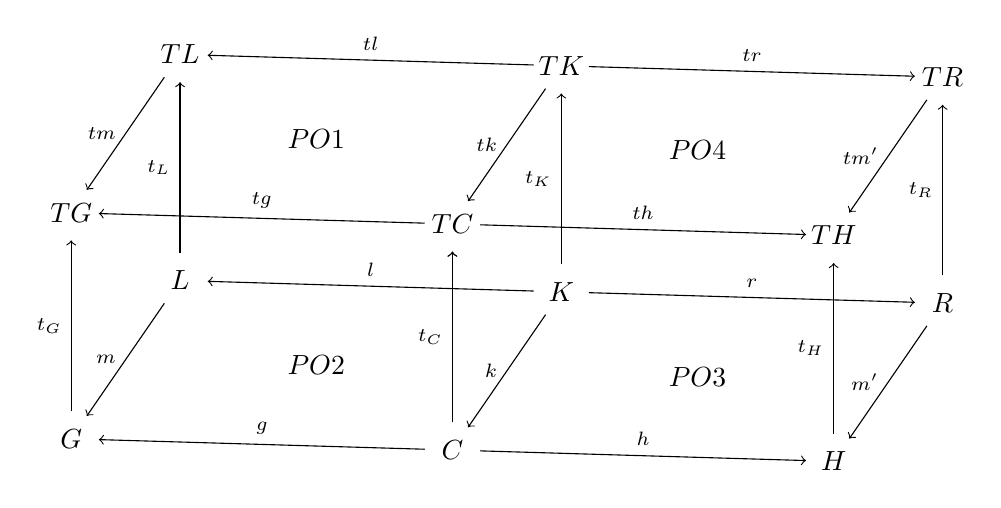
\begin{tikzpicture}[line join=round]
\draw[arrows=->  ,shorten >=10pt,shorten <=10pt](9.684,-.287)--(9.684,2.584);
\draw[arrows=->  ,shorten >=10pt,shorten <=10pt](3.459,-2.153)--(3.459,.718);
\draw[arrows=->  ,shorten >=10pt,shorten <=10pt](0,0)--(0,2.871);
\draw[arrows=->  ,shorten >=10pt,shorten <=10pt](4.842,-.144)--(4.842,2.727);
\draw[arrows=->  ,shorten >=10pt,shorten <=10pt](8.301,-2.297)--(8.301,.574);
\draw[arrows=->  ,shorten >=10pt,shorten <=10pt](3.459,-2.153)--(3.459,.718);
\draw[arrows=->  ,shorten >=10pt,shorten <=10pt](-1.383,-2.01)--(-1.383,.861);
\draw[arrows=->  ,shorten >=10pt,shorten <=10pt](4.842,-.144)--(9.684,-.287);
\draw[arrows=->  ,shorten >=10pt,shorten <=10pt](4.842,-.144)--(0,0);
\draw[arrows=->  ,shorten >=10pt,shorten <=10pt](3.459,-2.153)--(8.301,-2.297);
\draw[arrows=->  ,shorten >=10pt,shorten <=10pt](3.459,-2.153)--(-1.383,-2.01);
\draw[arrows=->  ,shorten >=10pt,shorten <=10pt](9.684,-.287)--(8.301,-2.297);
\draw[arrows=->  ,shorten >=10pt,shorten <=10pt](4.842,-.144)--(3.459,-2.153);
\draw[arrows=->  ,shorten >=10pt,shorten <=10pt](0,0)--(-1.383,-2.01);
\draw[arrows=->  ,shorten >=10pt,shorten <=10pt](4.842,2.727)--(9.684,2.584);
\draw[arrows=->  ,shorten >=10pt,shorten <=10pt](4.842,2.727)--(0,2.871);
\draw[arrows=->  ,shorten >=10pt,shorten <=10pt](3.459,.718)--(8.301,.574);
\draw[arrows=->  ,shorten >=10pt,shorten <=10pt](3.459,.718)--(-1.383,.861);
\draw[arrows=->  ,shorten >=10pt,shorten <=10pt](9.684,2.584)--(8.301,.574);
\draw[arrows=->  ,shorten >=10pt,shorten <=10pt](4.842,2.727)--(3.459,.718);
\draw[arrows=->  ,shorten >=10pt,shorten <=10pt](0,2.871)--(-1.383,.861);
\tikzstyle{angle}=[->,shorten >=15pt,shorten <=10pt]
\path (-1.383,-.574) node[left] {{\scriptsize$t_G$}}
               (0,1.435) node[left] {{\scriptsize$t_L$}} 
               (3.459,-.718) node[left] {{\scriptsize$t_C$}} 
               (4.842,1.292) node[left] {{\scriptsize$t_K$}} 
               (8.301,-.861) node[left] {{\scriptsize$t_H$}} 
               (9.684,1.148) node[left] {{\scriptsize$t_R$}};
        
\path (1.038,-2.081) node[above] {{\scriptsize$g$}}
                 (2.421,-.072) node[above] {{\scriptsize$l$}} 
                 (5.88,-2.225) node[above] {{\scriptsize$h$}} 
                 (7.263,-.215) node[above] {{\scriptsize$r$}};
          
\path (-.692,-1.005) node[left] {{\scriptsize$m$}}
                 (4.15,-1.148) node[left] {{\scriptsize$k$}} 
                 (8.992,-1.292) node[left] {{\scriptsize$m'$}};
          
\path (1.729,-1.077) node {$PO2$}
                 (6.571,-1.22) node {$PO3$};
          
\path (8.301,-2.297) node {$H$}
                 (9.684,-.287) node {$R$};
          
\path (3.459,-2.153) node {$C$}
                 (4.842,-.144) node {$K$};
          
\path (-1.383,-2.01) node {$G$}
                 (0,0) node {$L$};
          
\path (1.038,.789) node[above] {{\scriptsize$tg$}}
                 (2.421,2.799) node[above] {{\scriptsize$tl$}} 
                 (5.88,.646) node[above] {{\scriptsize$th$}} 
                 (7.263,2.656) node[above] {{\scriptsize$tr$}};
          
\path (-.692,1.866) node[left] {{\scriptsize$tm$}}
                 (4.15,1.722) node[left] {{\scriptsize$tk$}} 
                 (8.992,1.579) node[left] {{\scriptsize$tm'$}};
          
\path (1.729,1.794) node {$PO1$}
                 (6.571,1.651) node {$PO4$};
          
\path (8.301,.574) node {$TH$}
                 (9.684,2.584) node {$TR$};
          
\path (3.459,.718) node {$TC$}
                 (4.842,2.727) node {$TK$};
          
\path (-1.383,.861) node {$TG$}
                 (0,2.871) node {$TL$};
          
\end{tikzpicture}% End sketch output

    \end{center}
      \vspace*{-1cm}
    \caption{Co-transformation}
    \label{fig:co-transformation}
\end{figure}

\section{Double-Cube Top}
\begin{figure}[ht]
\begin{minipage}[b]{0.33\linewidth}
\centering
   \fbox{\includegraphics[max size={0.9\textwidth}{0.9\textheight}]{TL}}
\caption{TL}
\label{fig:figure1}
\end{minipage}
\hspace{0.5cm}
\begin{minipage}[b]{0.33\linewidth}
\centering
   \fbox{\includegraphics[max size={0.9\textwidth}{0.9\textheight}]{TK}}
\caption{TK}
\label{fig:figure2}
\end{minipage}
\begin{minipage}[b]{0.33\linewidth}
\centering
   \fbox{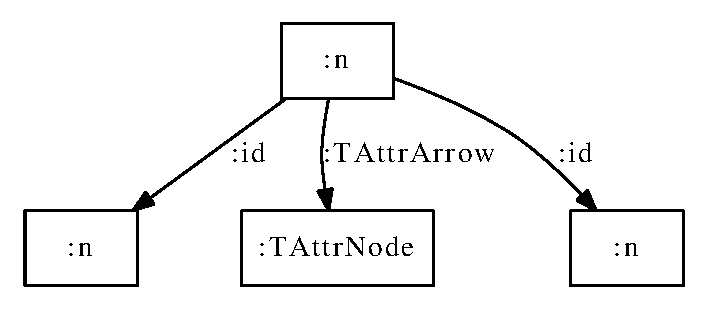
\includegraphics[max size={0.9\textwidth}{0.9\textheight}]{TR}}
\caption{TR}
\label{fig:figure1}
\end{minipage}
\begin{minipage}[b]{0.33\linewidth}
\centering
   \fbox{\includegraphics[max size={0.9\textwidth}{0.9\textheight}]{TG}}
\caption{TG}
\label{fig:figure1}
\end{minipage}
\hspace{0.5cm}
\begin{minipage}[b]{0.33\linewidth}
\centering
   \fbox{\includegraphics[max size={0.9\textwidth}{0.9\textheight}]{TC}}
\caption{TC}
\label{fig:figure2}
\end{minipage}
\begin{minipage}[b]{0.33\linewidth}
\centering
   \fbox{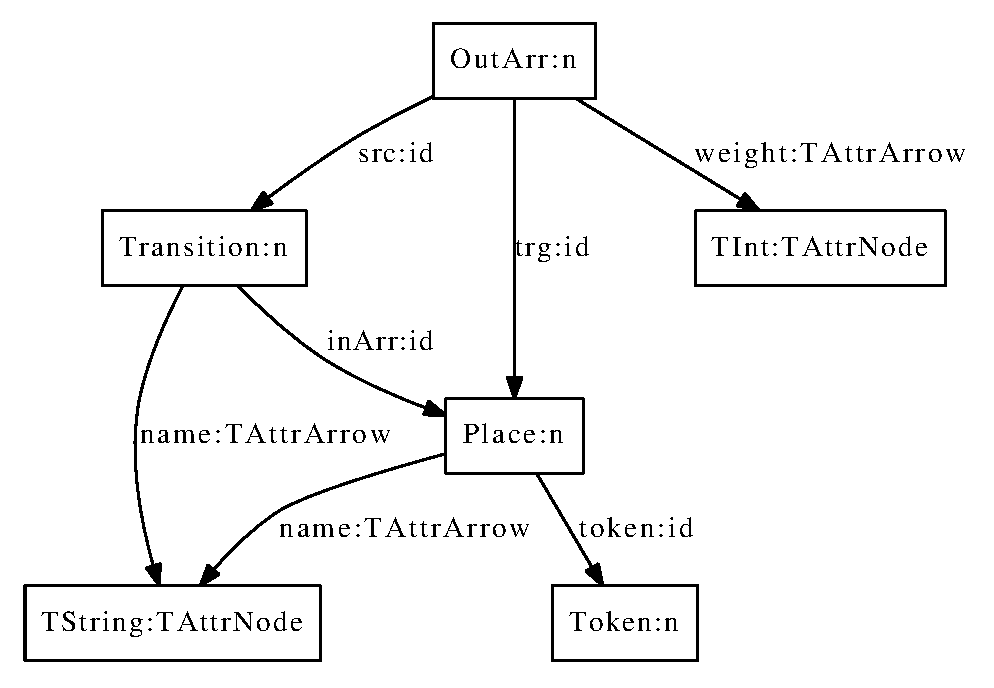
\includegraphics[max size={0.9\textwidth}{0.9\textheight}]{TH}}
\caption{TH}
\label{fig:figure1}
\end{minipage}
\end{figure}


\section{Double-Cube Bottom}

\begin{figure}[ht]
\begin{minipage}[b]{0.33\linewidth}
\centering
   \fbox{\includegraphics[max size={0.9\textwidth}{0.9\textheight}]{L}}
\caption{L}
\label{fig:figure1}
\end{minipage}
\hspace{0.5cm}
\begin{minipage}[b]{0.33\linewidth}
\centering
   \fbox{\includegraphics[max size={0.9\textwidth}{0.9\textheight}]{K}}
\caption{K}
\label{fig:figure2}
\end{minipage}
\begin{minipage}[b]{0.33\linewidth}
\centering
   \fbox{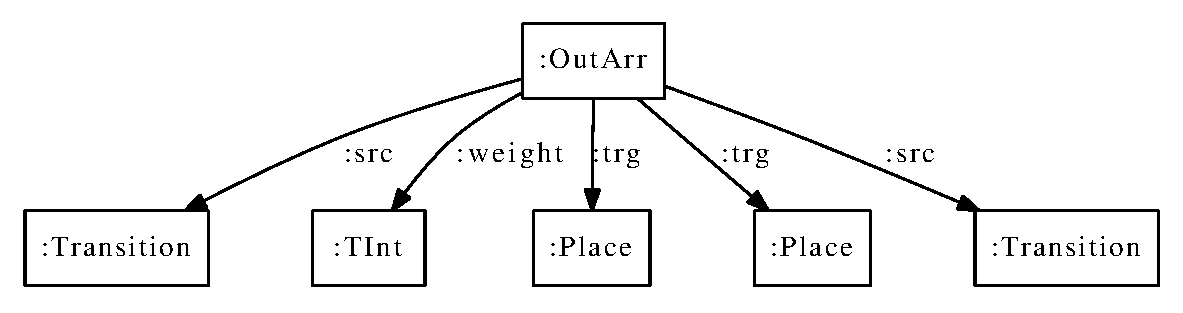
\includegraphics[max size={0.9\textwidth}{0.9\textheight}]{R}}
\caption{R}
\label{fig:figure1}
\end{minipage}
\begin{minipage}[b]{0.33\linewidth}
\centering
   \fbox{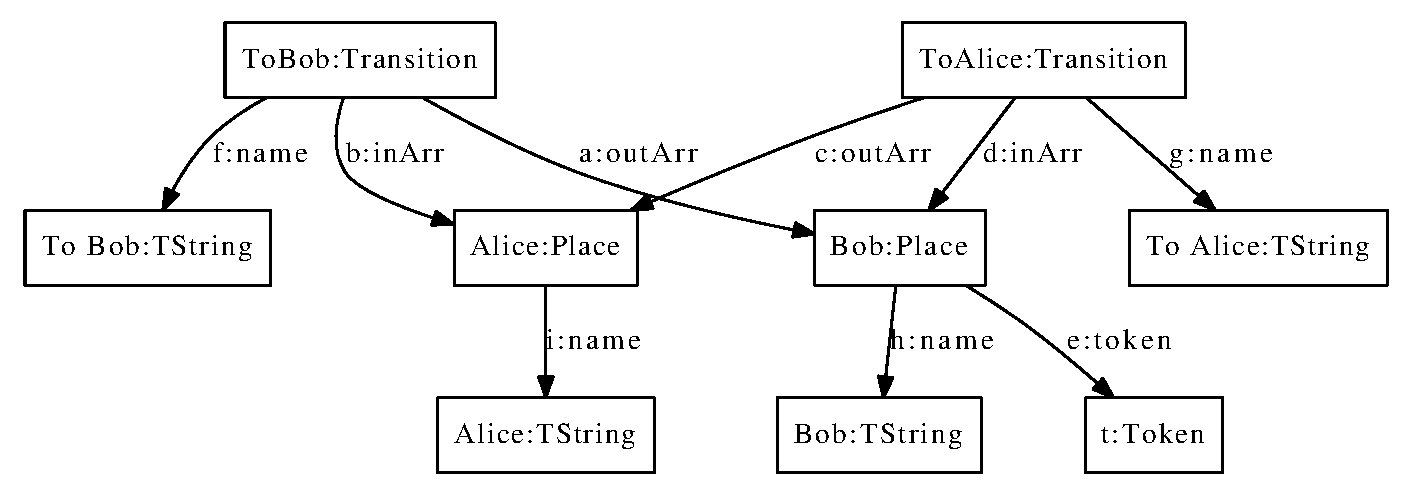
\includegraphics[max size={0.9\textwidth}{0.9\textheight}]{G}}
\caption{G}
\label{fig:figure1}
\end{minipage}
\hspace{0.5cm}
\begin{minipage}[b]{0.33\linewidth}
\centering
   \fbox{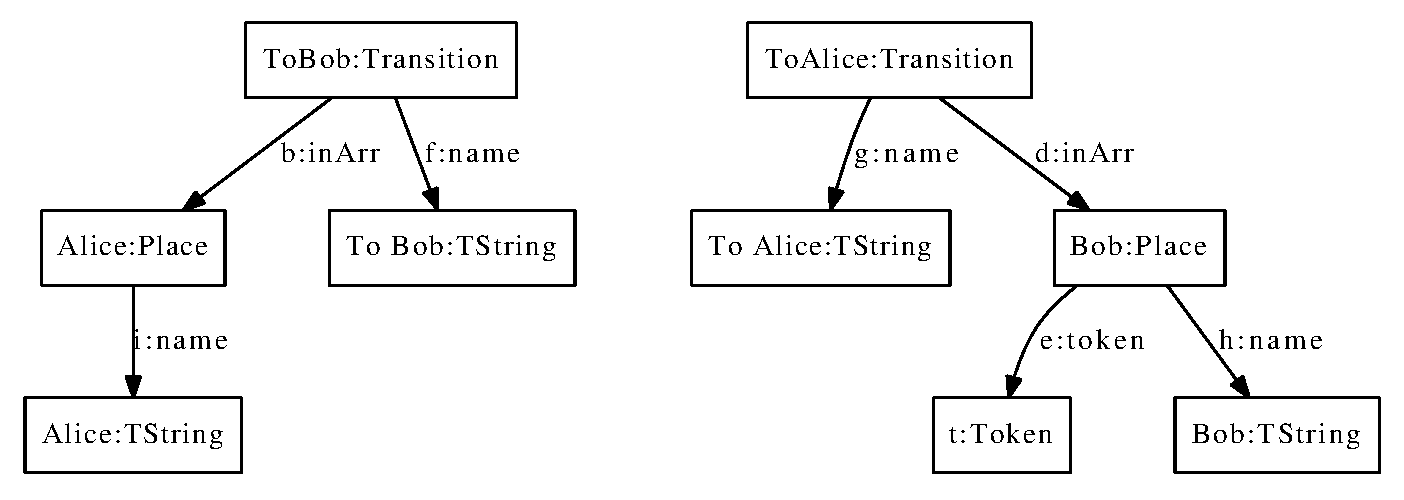
\includegraphics[max size={0.9\textwidth}{0.9\textheight}]{C}}
\caption{C}
\label{fig:figure2}
\end{minipage}
\begin{minipage}[b]{0.33\linewidth}
\centering
   \fbox{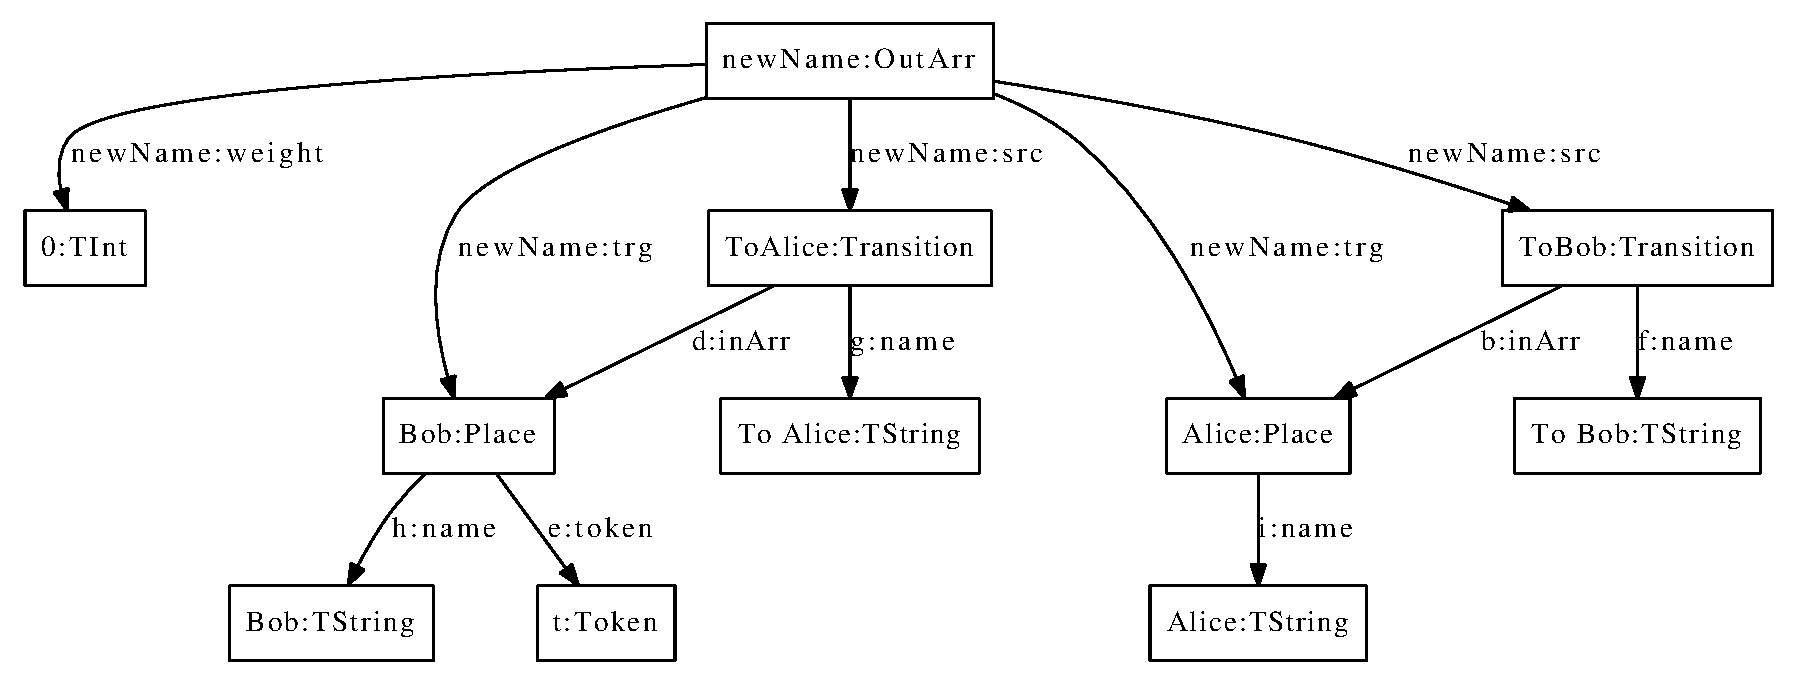
\includegraphics[max size={0.9\textwidth}{0.9\textheight}]{H}}
\caption{H}
\label{fig:figure1}
\end{minipage}
\end{figure}

\end{landscape}


\section{Graph TL}

\begin{figure}[h!]
  \centering
    \includegraphics[max size={\textwidth}{\textheight}]{TL}
  \caption{TL}
\end{figure}

\section{Graph TK}

\begin{figure}[h!]
  \centering
    \includegraphics[max size={\textwidth}{\textheight}]{TK}
  \caption{TK}
\end{figure}

\section{Graph TR}

\begin{figure}[h!]
  \centering
    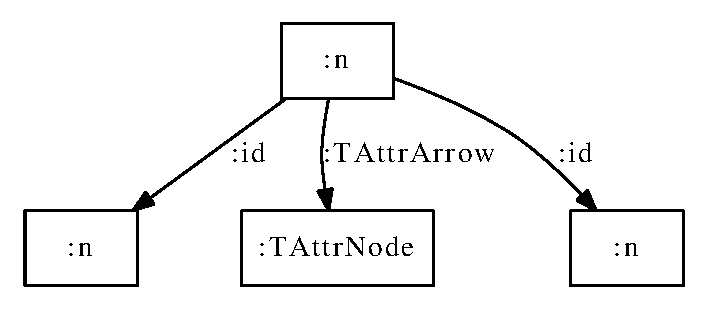
\includegraphics[max size={\textwidth}{\textheight}]{TR}
  \caption{TR}
\end{figure}

\section{Graph TG}

\begin{figure}[h!]
  \centering
    \includegraphics[max size={\textwidth}{\textheight}]{TG}
  \caption{TG}
\end{figure}

\section{Graph TC}

\begin{figure}[h!]
  \centering
    \includegraphics[max size={\textwidth}{\textheight}]{TC}
  \caption{TC}
\end{figure}


\section{Graph TH}

\begin{figure}[h!]
  \centering
    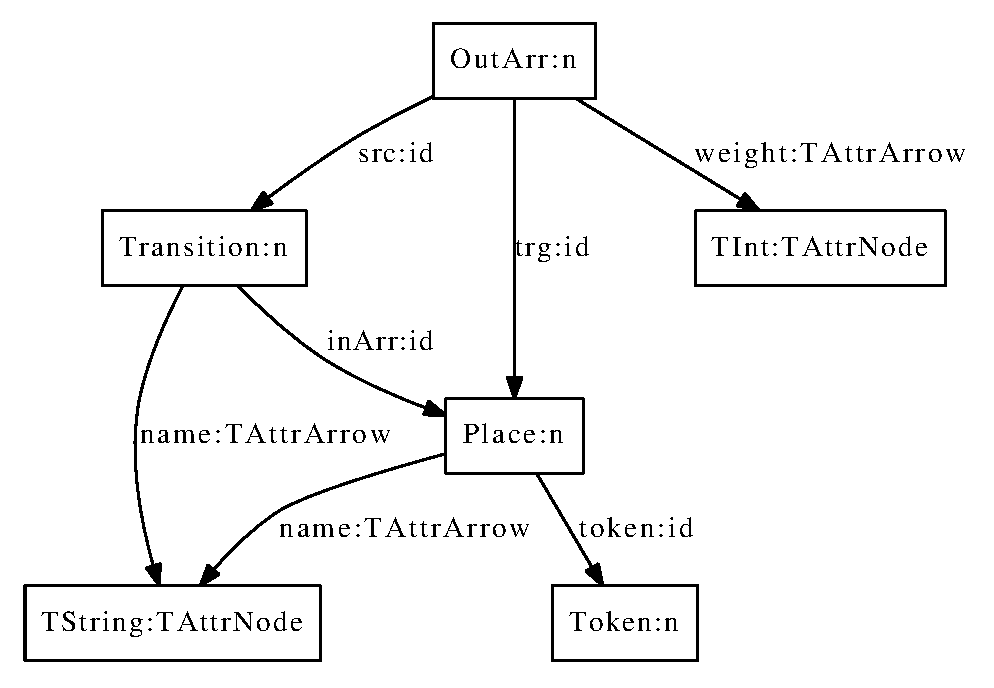
\includegraphics[max size={\textwidth}{\textheight}]{TH}
  \caption{TH}
\end{figure}


\section{Graph L}

\begin{figure}[h!]
  \centering
    \includegraphics[max size={\textwidth}{\textheight}]{L}
  \caption{L}
\end{figure}

\section{Graph K}

\begin{figure}[h!]
  \centering
    \includegraphics[max size={\textwidth}{\textheight}]{K}
  \caption{K}
\end{figure}

\section{Graph R}

\begin{figure}[h!]
  \centering
    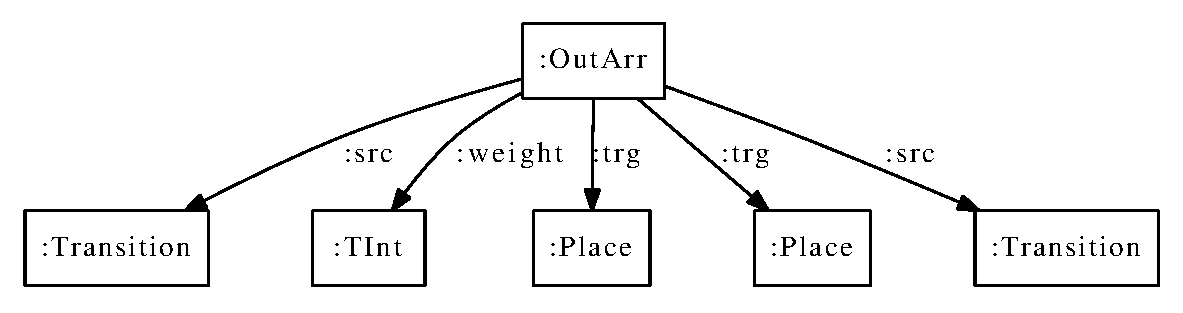
\includegraphics[max size={\textwidth}{\textheight}]{R}
  \caption{R}
\end{figure}

\section{Graph G}

\begin{figure}[h!]
  \centering
    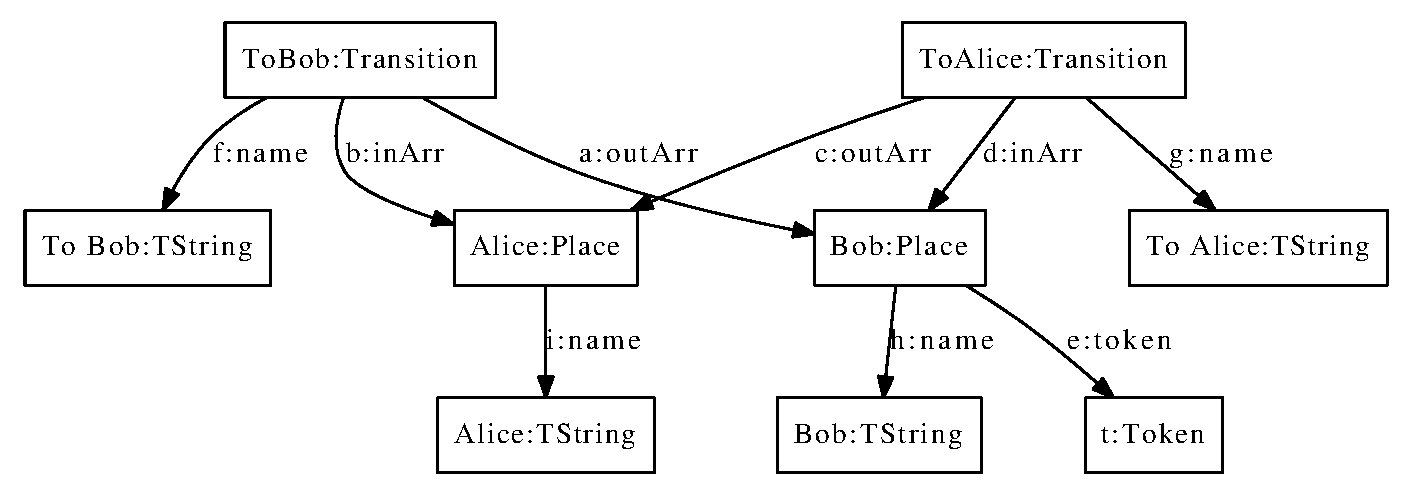
\includegraphics[max size={\textwidth}{\textheight}]{G}
  \caption{G}
\end{figure}

\section{Graph C}

\begin{figure}[h!]
  \centering
    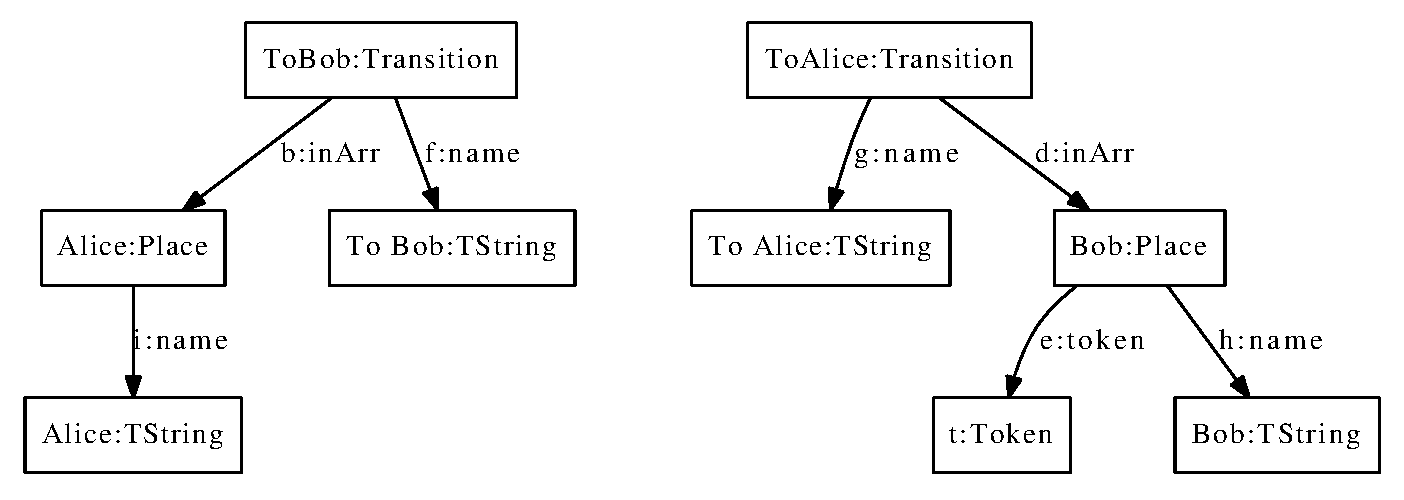
\includegraphics[max size={\textwidth}{\textheight}]{C}
  \caption{C}
\end{figure}


\section{Graph H}

\begin{figure}[h!]
  \centering
    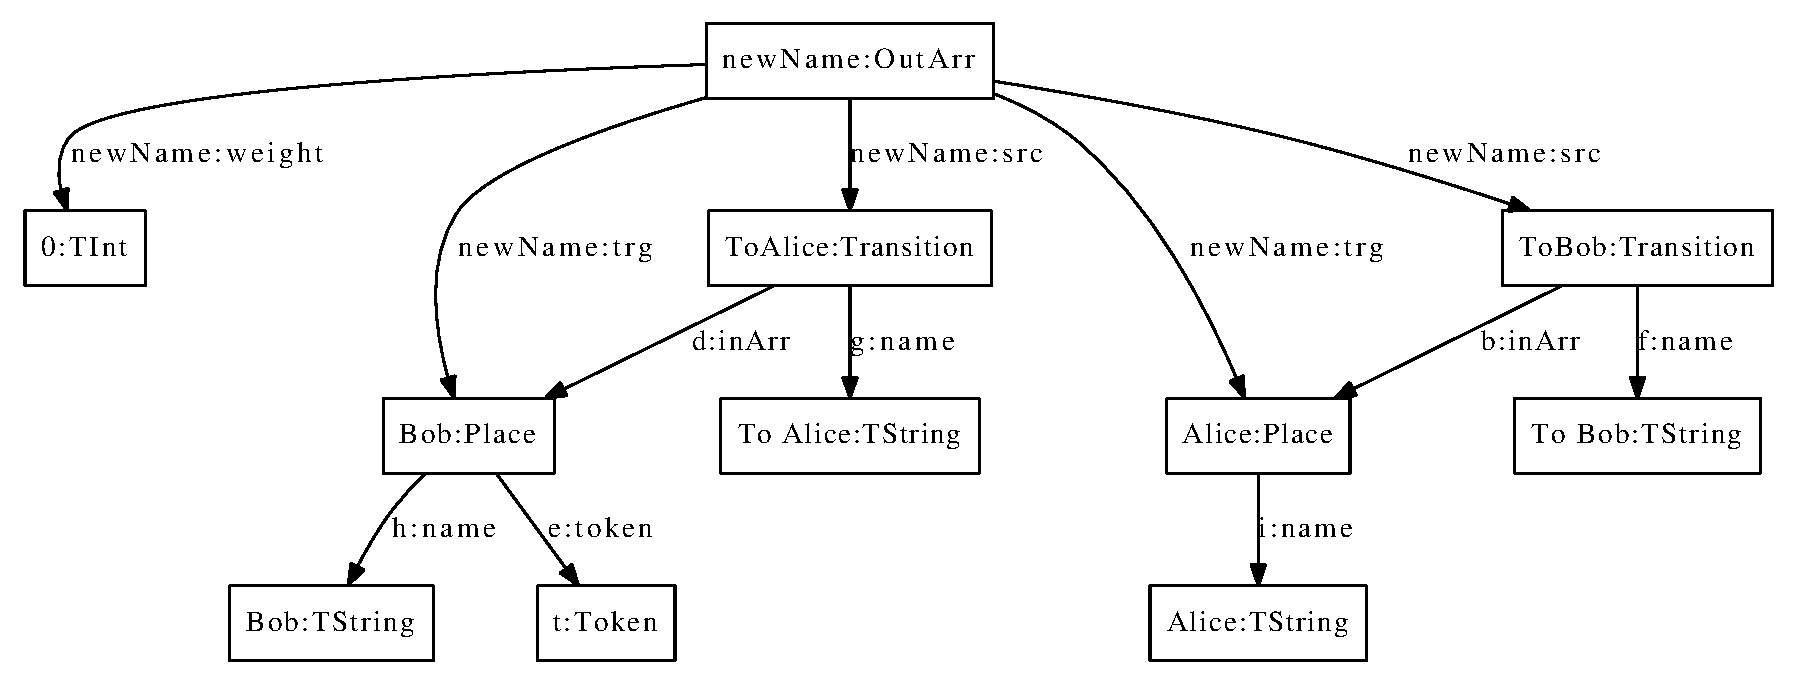
\includegraphics[max size={\textwidth}{\textheight}]{H}
  \caption{H}
\end{figure}

\end{document} 
